\documentclass[12pt]{article}
\usepackage{polski}
\usepackage{lmodern}
\usepackage[utf8]{inputenc}
\usepackage{tabto}
\usepackage{indentfirst} %pierwszy akapit posiada wcięcie
\usepackage{graphicx} 
\title{Interpolacja wielomianowa - projekt}
\author{Natalia Wojtania i Grzegorz Chojnacki}
%\date{}
\begin{document}
\maketitle

\section{Zadanie}
\subsection{Tytuł}
Tytuł zadania to "Dwutlenek węgla".
\subsection{Treść}
Program,  który  oszacuje  tempo  przyrostu dwutlenku węgla w atmosferze Ziemi. Węzły mają  przedstawiać  ilość  wyemitowanego  do atmosfery $ CO_{2}$ w  ciągu  roku  lub  w  innym przedziale czasowym.
\subsection{Metoda}
W programie należy wykorzystać metodę Newtona.
\subsubsection{Opis metody}
Mając zadany układ punktów $\{(x_{j},y_{j}),j=0,1,2,3...,n\}$, gdzie $x_{0},x_{1},x_{2},...,x_{n}$ są węzłami interpolacyjnymi, a $y_{0},y_{1},...,y_{n}$ wartościami, poszukujemy wielomianu interpolacyjnego $P \in \sqcap_{n}$ spełniającego warunki $P(x_{i})=y_{i}, i=0,1,2,...,n$ w postaci :
$$ P(x)=b_{0}+b_{1}(x-x_{0})+b_{2}(x-x_{0})(x-x_{1})+...+b_{n}(x-x_{0})\cdot...\cdot(x-x_{n-1}).$$
Z wyżej wymienionych warunków otrzymamy układ z niewiadomymi $b_{0},b_{1},...,b_{n}.$ 
Z pierwszego równania $P(x_{0})=y_{0}=b_{0}$, następnie $P(x_{1})=y_{1}=b_{0}+b_{1}(x-x_{0})$, stąd $b_{1}=\frac{y_{1}-y_{0}}{x_{1}-x_{0}}$ itd.
\subsubsection{Przykład}
\begin{tabular}{c|c|c|c}
$x_{i}$&0&2&3 \\ \hline
$y_{i}$&1&11&19
\end{tabular}
\hspace{10mm} $ P(x)=b_{0}+b_{1}(x-0)+b_{2}(x-0)(x-2)$
\\ \\
Z warunku $P(0)=1$ mamy $ b_{0}=1,$ z $P(2)=11$ mamy $b_{1}=5,$ z $ P(3)=19 $ mamy $ b_{2}=1.$
\\Stąd $P(x)=1+5(x-0)+1(x-0)(x-2)=x^{2}+3x+1.$
\section{Opis implementacji algorytmu}
Implementacja realizująca metodę Newtona.
\subsection{Dane wejściowe}
Na wejściu program pobiera od użytkownika wartości punktów \\$P_{j}(x,y), j=0,1,2,...,n$, gdzie 'Rok pomiarów' to x, a 'Przyrost $ CO_{2}$ [Mt]' to y. Realizacja wprowadzenia danych możliwa jest na dwa sposoby. Poprzez bezpośrednie wpisanie wartości lub zaimportowanie danych z pliku JSON.
\subsection{Struktury danych}
Każdy wielomian to lista współczynników, gdzie poszczególny indeks odpowiada potędze $x$ przy danym współczynniku. Zerowy element obrazuje $ x^{0} $($x$ do potęgi zerowej), pierwszy element odpowiada $ x^{1} $ itd. 
\begin{description}
 
 \item[PRZYKŁAD]:\hspace{5 mm}  [2,-1,2,-2] oznacza $-2x^{3} + 2x^{2} - x + 2$.
 \\
\end{description}
\subsubsection{Wielomian}Program korzysta ze struktury klasy \emph{Polynomial}, która wspiera operacje:
\begin{itemize}
 \item Dodawanie: Przewidziane dla wyrazów wolnych jak i wielomianów. Odpowiednie elementy list obu wielomianów są dodawane.
 \begin{description}
 
 \item[PRZYKŁAD]:\hspace{5 mm}[0, 0, 3] + [1, 2, 0, 4] = [1, 2, 3, 4] \\ oznacza 
  $3x^2 + 4x^{3}+2x+1 = 4x^{3}+3x^{2}+2x+1 $
   \end{description}
 \item Mnożenie: Podczas mnożenia razy $x^{n}$ ($x$ do potęgi n-tej) każdy wykładnik jest podnoszony o potęgę $n$, a lista przesuwa się o $n$ miejsc. W przypadku mnożenia wielomianu razy wielomian, drugi wielomian mnożymy przez każdy składnik pierwszego i sumujemy.
 \begin{description}
 
\item[PRZYKŁAD]:\hspace{5 mm}[3, 3] $\cdot$ [-3, 3] = [-9,0,9] \\ oznacza $(3x + 3)(3x - 3) = 9x^{2} - 9$
 \end{description}
 \item Wyliczanie wartości w punkcie: Za pomocą metody Hornera.
\end{itemize}
\subsubsection{Punkt}
Wykorzystywane są również proste obiekty modelujące punkty. Zawierają tylko 2 pola x i y.
\subsection{Funkcje pomocnicze}

W programie wykorzystywane są takie funkcje jak:
\begin{enumerate}
\item map: transformacja każdego elementu danej listy 
\item reduce: sprowadzenie listy do pojedynczej wartośći, przy pomocy funkcji działającej na kolejnych elementach danej listy 
\item filter: filtrowanie danych w liście, spełniających określony warunek
\end{enumerate}
\subsection{Przebieg działania}
Program wyświetla komunikat: 'Wprowadź listę punktów poniżej'. Jeśli zostały wprowadzone prawidłowe dane, to na bieżąco wyświetlany jest odpowiedni wielomian. 
Próba ręcznego wprowadzenia nieprawidłowych danych, które weryfikowane są w programie poprzez funkcję \emph{getPoints} skutkuje zignorowaniem błędnego punktu. Podobnie dzieje się w sytuacji pozostawienia pustego pola.
Program sprawdza czy 'Rok pamiarów' nie powtarza się.
\par Dane dostarczone z pliku JSON program sprawdza poprzez funkcję \emph{parsePoints} oraz wyświetla komunikat "Błąd wczytywania pliku" w przypadku niepowodzenia.\\
\par Następnie funkcja \emph{recalculate} zajmuje się przekazaniem punktów, w celu dalszego rachunku, a także wyświetleniem wyniku.\\
Funkcja \emph{getPolynomial} klasy \emph{NewtonEvaluator} zwraca wielomian, licząc wcześniej niewiadome $b_0$, $b_1$...; mając tylko jeden punkt zwracana jest od razu wartość y. W przeciwnym wypadku zwracany jest wyliczany wielomian. 
\\
Z listy punktów generowana jest lista list, która przypomina piramidę, gdzie każda lista zawiera o jeden element mniej.
Każda lista stanowi grupę punktów, na podstawie których wyliczane są niewiadome $b_0,b_1,...,b_n$.\\
$$b_{n}=\frac{y_{n}-P(x_{n-1})} { (x_n-x_0)(x_n-x_1)...(x_n-x_{n-1})} $$\\
$$P(x_{n})=b_{0}-b_{1}(x_n-x_{0})-b_2(x_n-x_0)(x_n-x_1)-...-b_{n-1}(x_n-x_0)(x_n-x_1)...(x_n-x_{n-1})$$

Wykorzystywane są funkcje rekurencyjne \emph{getB} oraz \emph{P} , w których przypadkiem bazowym jest lista z jednym punktem, dla której zwracana jest wartość y tego punktu. W przeciwnym wypadku obie te funkcje dostają listę punktów do xn i wyliczają wyniki na podstawie powyższych wzorów. Korzystają z funkcji pomocnicznej \emph{pointProduct}, która przekształca listę punktów na listę wielomianów w postaci $x_n \rightarrow (x-x_n)$. Następnie wylicza ich iloczyn. 

Aby wyznaczyć wielomian musimy zsumować niewiadomą $b_0$ i iloczyn pozostałych niewiadomych z odpowiadającymi im grupami wielomianowymi. 

Z uwagi na występowanie rekurencji i dużą powtarzalność wykonywanych operacji
w najbardziej kluczowych fragmentach, wykorzystywana jest technika spamiętywania.
\\ \\
Wynikiem działania programu jest wielomian interpolacyjny () obrazujący oszacowanie tempa przyrostu dwutlenku węgla.
\newpage
\subsection{Najważniejsze fragmenty programu}
newtonEvaluator.js
\begin{verbatim}

class NewtonEvaluator {
  constructor(points) { this.points = points }

  getPolynomial() {
    if (this.points.length === 1) return new Polynomial([this.points[0].y])

    const [b0, ...bs] = this.getBs()
    const polynomials = init(this.points)
      .map(Polynomial.point)
      .map(getListSlicesFromStart)
      .map(group => group.reduce(Polynomial.product))

    return polynomials
      .map((polynomial, index) => polynomial.multiply(bs[index]))
      .reduce(Polynomial.sum)
      .add(b0)
  }

  getBs() {
    const pointProduct = (points) => points
      .map(Polynomial.point)
      .reduce(Polynomial.product)

    const P = memoized((points) => {
      if (points.length === 1) return new Polynomial([points[0].y])
      else {
        const rest = init(points)
        return P(rest).add(pointProduct(rest).multiply(getB(points)))
      }
    })

    const getB = memoized((points) => {
      if (points.length === 1) return points[0].y
      else {
        const [current, rest] = [last(points), init(points)]
        return (current.y - P(rest).at(current.x)) /
         pointProduct(rest).at(current.x)
      }
    })

    return this.points.map(getListSlicesFromStart).map(getB)
  }
}

\end{verbatim}
polynomial.js
\begin{verbatim}

class Polynomial {
  static one  = new Polynomial([1])
  static zero = new Polynomial([0])
  static point = (p) => new Polynomial([-p.x, 1])
  static product = (acc, polynomial) => acc.multiply(polynomial)
  static sum     = (acc, polynomial) => acc.add(polynomial)

  terms = []

  constructor(terms) {
    const trimmed = terms => {
      if (terms.length === 0) return [0]
      else if (last(terms) !== 0) return terms
      else return trimmed(init(terms))
    }

    if (terms.length === 0) throw new Error('Term list is empty')
    else this.terms = trimmed(terms)
  }

  at(x) {
    return this.terms.reduceRight((acc, term) => acc * x + term)
  }

  add(that) {
    if (typeof that == 'number') return this.addNumber(that)
    else return this.addPolynomial(that)
  }

  addNumber(that) {
    const [head, ...tail] = this.terms
    return new Polynomial([head + that, ...tail])
  }

  addPolynomial(that) {
    const [longer, shorter] = (this.terms.length >= that.terms.length)
    ? [this, that]
    : [that, this]

    
    const addedTerms = zip(longer.terms, shorter.terms).map(pairSum)

    return new Polynomial(addedTerms)
  }

  multiply(that) {
     
    const padLeft = (arr, padding) => new Array(padding).fill(0).concat(arr)

    const multiplyByTerm = (thisTerm, power, that) => {
      const multiplied = that.terms.map(thatTerm => thatTerm * thisTerm)
      return padLeft(multiplied, power)
    }

    if (typeof that === "number") return this.multiply(new Polynomial([that]))
    else return this.terms
      .map((term, power) => multiplyByTerm(term, power, that))
      .map(terms => new Polynomial(terms))
      .reduce(Polynomial.sum)
  }

}
\end{verbatim}

\subsection{Widok działania programu}
\begin{figure}[h]
\centering
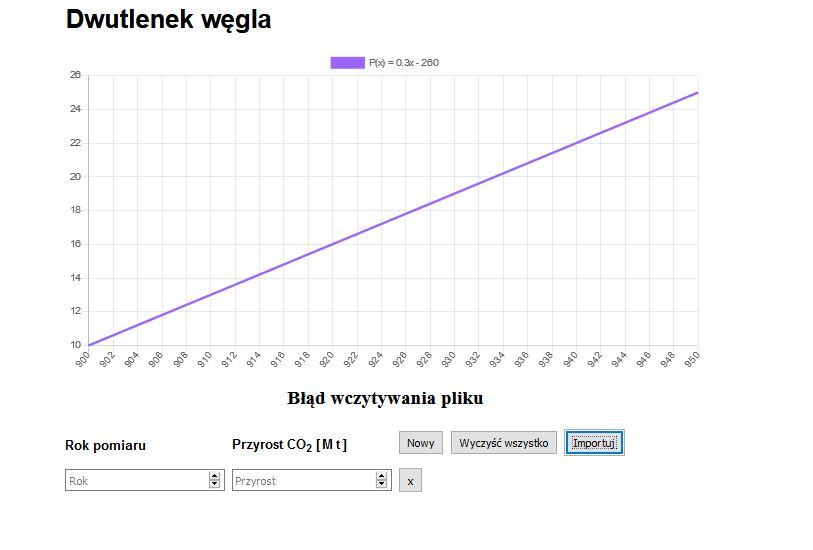
\includegraphics[scale=0.65]{errorPic.jpg}
\caption{Błędne zaimportowanie pliku}
\end{figure}

\begin{figure}
\centering
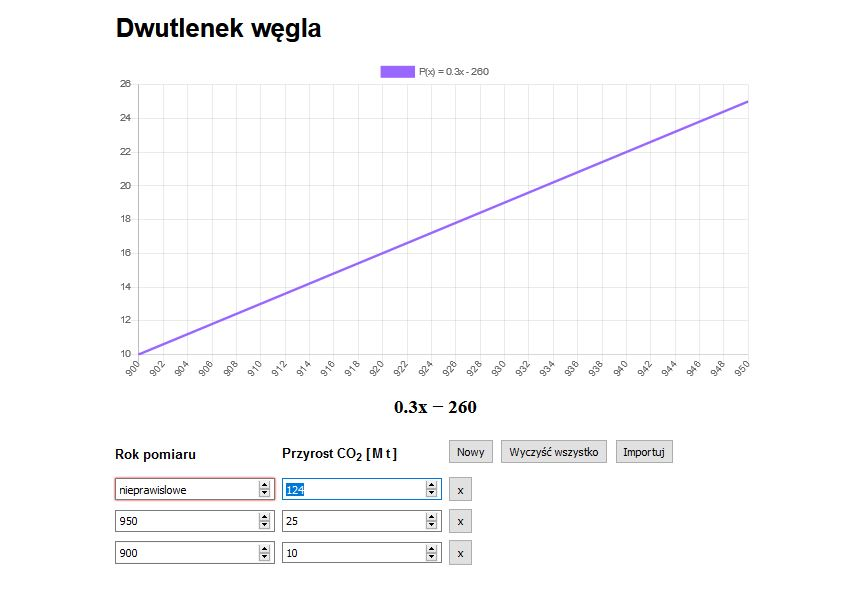
\includegraphics[scale=0.65]{wrongInput.jpg}
\caption{Nieprawidłowo wprowadzone dane}
\end{figure}
\begin{figure}
\centering
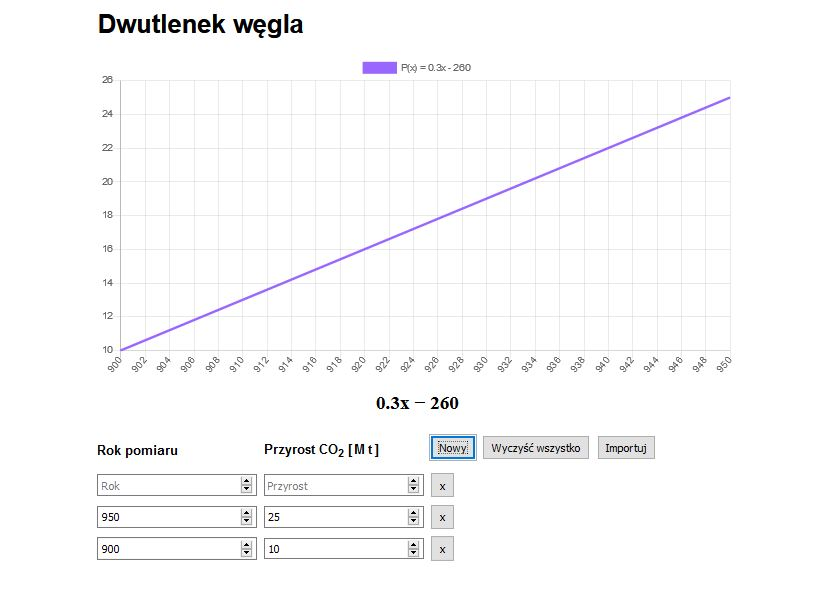
\includegraphics[scale=0.65]{emptyInput.jpg}
\caption{Ignorowane puste pole}
\end{figure}

\begin{figure}
\centering
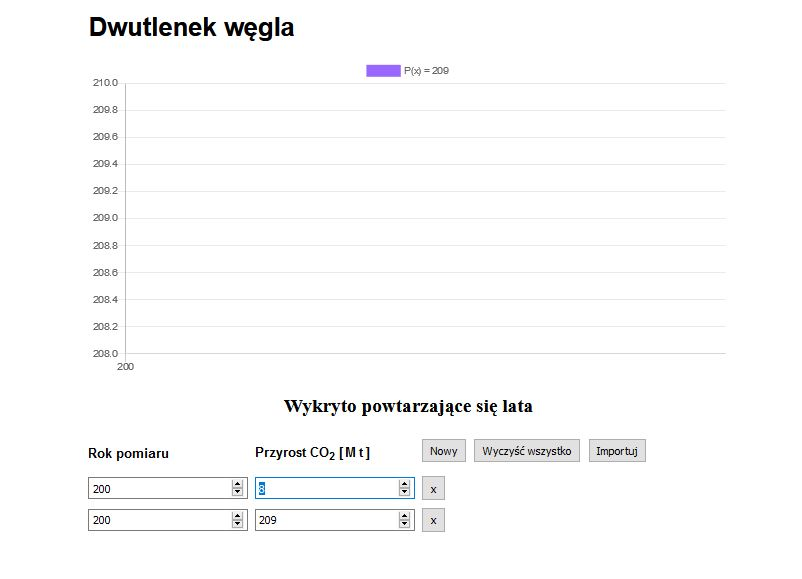
\includegraphics[scale=0.65]{duplicate.jpg}
\caption{Duplikat}
\end{figure}

\begin{figure}
\centering
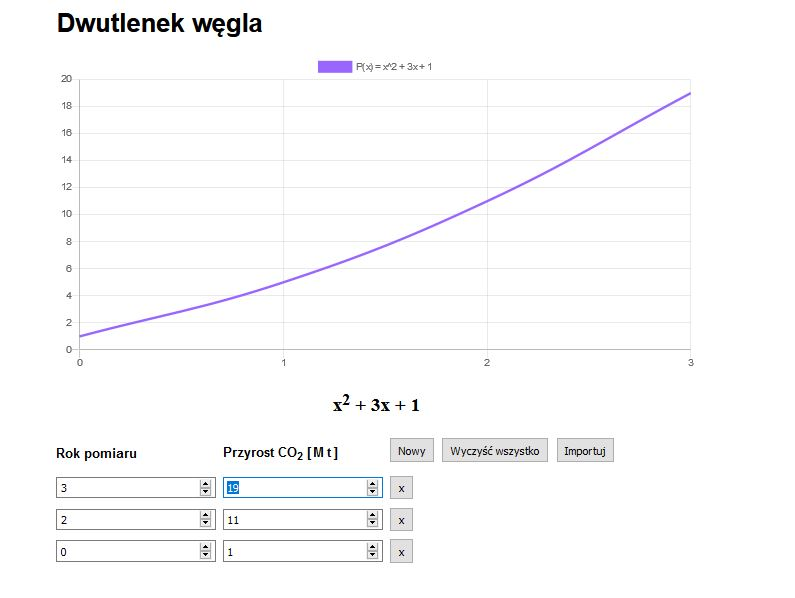
\includegraphics[scale=0.65]{correctEasyData.jpg}
\caption{Przykład opisany w dokumencie}
\end{figure}

\begin{figure}
\centering
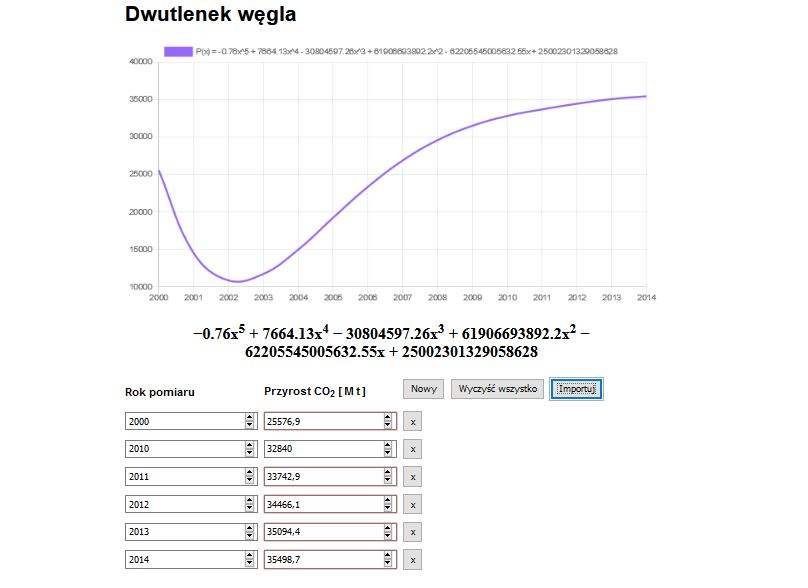
\includegraphics[scale=0.65]{correctRealData.jpg}
\caption{Przykład z rzeczywistymi danymi}
\end{figure}

%file:///C:/Users/HP/AppData/Local/Temp/W1_Interpolacja%20wielomianowa.pdf
\end{document}